
\documentclass[10pt]{beamer}
\usetheme{metropolis}

% ── Packages ──
\usepackage{amsmath,amssymb,amsthm}
\usepackage{tikz}
\usetikzlibrary{positioning,arrows.meta,fit,matrix,backgrounds,calc,shapes.geometric}
\usepackage{graphicx}
\usepackage{array}
\usepackage{etoolbox}

% ── Theorem environments ──
\theoremstyle{definition}
\newtheorem{defi}{Definition}[section]
\newtheorem{prop}{Proposition}[section]
\newtheorem{thm}{Theorem}[section]
\newtheorem{cor}{Corollary}[section]

% Custom theorem styles with colors
\setbeamercolor{block title}{bg=red!75!black,fg=white}
\setbeamercolor{block body}{bg=yellow!10!white}

\AtBeginEnvironment{prop}{%
  \setbeamercolor{block title}{bg=yellow!75!black,fg=black}%
  \setbeamercolor{block body}{bg=yellow!10!white}%
}
\AtEndEnvironment{prop}{%
  \setbeamercolor{block title}{bg=red!75!black,fg=white}%
}

\AtBeginEnvironment{thm}{%
  \setbeamercolor{block title}{bg=yellow!75!black,fg=black}%
  \setbeamercolor{block body}{bg=yellow!10!white}%
}
\AtEndEnvironment{thm}{%
  \setbeamercolor{block title}{bg=red!75!black,fg=white}%
}

\AtBeginEnvironment{cor}{%
  \setbeamercolor{block title}{bg=yellow!75!black,fg=black}%
  \setbeamercolor{block body}{bg=yellow!10!white}%
}
\AtEndEnvironment{cor}{%
  \setbeamercolor{block title}{bg=red!75!black,fg=white}%
}

% ── Highlighting ──
\newcommand{\x}[1]{\alert{\textbf{#1}}}

% ── Cross-filling colors ──
\newcommand{\pvt}[1]{{\color{red}\mathbf{#1}}}       % pivot
\newcommand{\crs}[1]{{\color{blue}#1}}                % cross arm

\title{Lecture 9: Compatible Projections}
\subtitle{MATH203 Applied Linear Algebra}
\date{}
\titlegraphic{}

\begin{document}
\maketitle

% ═══════════════════════════════════════
% §1 REVIEW: WHAT CROSS-FILLING DISCOVERED
% ═══════════════════════════════════════
\section{Review: What Cross-Filling Discovered}

\begin{frame}{Recall from Lecture 8}

We cross-filled a projection $P = P^2$:

$$P = \underbrace{\begin{pmatrix} 0 & 0 & 0 \\ -1 & 1 & 0 \\ 0 & 0 & 0 \end{pmatrix}}_{R_1} + \underbrace{\begin{pmatrix} 0 & 0 & 0 \\ 0 & 0 & 0 \\ -1 & 0 & 1 \end{pmatrix}}_{R_2}$$

\vspace{0.5em}

We discovered two \x{remarkable} properties:

\begin{enumerate}
\item Each $R_i$ is a projection: $R_1^2 = R_1$, $R_2^2 = R_2$
\item Mutual annihilation: $R_1 R_2 = 0$, $R_2 R_1 = 0$
\end{enumerate}

\end{frame}

\begin{frame}{The Two Properties Together}

Property 1 alone is not special --- many matrices satisfy $R^2 = R$.

\vspace{0.5em}

Property 2 alone is not special --- many pairs satisfy $AB = 0$.

\vspace{0.5em}

But \x{together} they form a remarkable structure:

\vspace{0.5em}

\begin{itemize}
\item Each $R_i$ projects onto its own ``floor''
\item $R_i R_j = 0$ means: the floor of $R_j$ lies entirely in the \x{sunlight direction} of $R_i$
\end{itemize}

\vspace{0.5em}

\x{Today}: We name this structure, prove a stunning theorem about it, and discover powerful decomposition methods.

\end{frame}


% ═══════════════════════════════════════
% §2 COMPATIBLE FAMILIES OF PROJECTIONS
% ═══════════════════════════════════════
\section{Compatible Families}

\begin{frame}{Definition}

\begin{defi}[Compatible Family]
A collection of projections $\{P_1, P_2, \ldots, P_k\}$ (each satisfying $P_i^2 = P_i$) is called a \x{compatible family} if:
$$P_i P_j = 0 \quad \text{for all } i \neq j$$
\end{defi}

\end{frame}

\begin{frame}{Example: Coordinate Projections in $\mathbb{R}^3$}

$$P_1 = \begin{pmatrix} 1 & 0 & 0 \\ 0 & 0 & 0 \\ 0 & 0 & 0 \end{pmatrix}, \quad P_2 = \begin{pmatrix} 0 & 0 & 0 \\ 0 & 1 & 0 \\ 0 & 0 & 0 \end{pmatrix}, \quad P_3 = \begin{pmatrix} 0 & 0 & 0 \\ 0 & 0 & 0 \\ 0 & 0 & 1 \end{pmatrix}$$

\vspace{0.5em}

Check: each is a projection ($P_i^2 = P_i$ $\checkmark$)

\vspace{0.5em}

Check: $P_1 P_2 = 0$, $P_1 P_3 = 0$, $P_2 P_3 = 0$ $\checkmark$

\vspace{0.5em}

Bonus: $P_1 + P_2 + P_3 = I_3$

\end{frame}

\begin{frame}[fragile]{Geometric Picture: Coordinate Projections}

\begin{center}
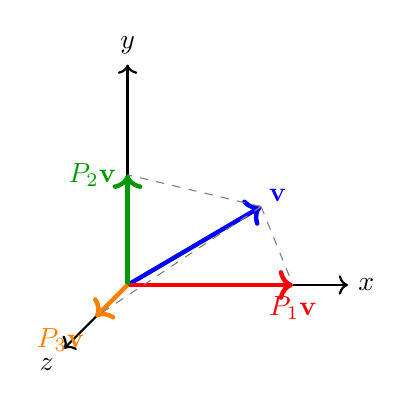
\begin{tikzpicture}[scale=0.7]
% Axes
\draw[->,thick] (0,0,0) -- (4,0,0) node[right]{$x$};
\draw[->,thick] (0,0,0) -- (0,4,0) node[above]{$y$};
\draw[->,thick] (0,0,0) -- (0,0,3) node[below left]{$z$};
% Vector v
\draw[->,ultra thick, blue] (0,0,0) -- (3,2,1.5);
\node[blue] at (3.3,2.2,1.5) {$\mathbf{v}$};
% Projections
\draw[->,ultra thick, red] (0,0,0) -- (3,0,0) node[below]{$P_1\mathbf{v}$};
\draw[->,ultra thick, green!60!black] (0,0,0) -- (0,2,0) node[left]{$P_2\mathbf{v}$};
\draw[->,ultra thick, orange] (0,0,0) -- (0,0,1.5) node[below left]{$P_3\mathbf{v}$};
% Dashed
\draw[dashed,gray] (3,2,1.5) -- (3,0,0);
\draw[dashed,gray] (3,2,1.5) -- (0,2,0);
\draw[dashed,gray] (3,2,1.5) -- (0,0,1.5);
\end{tikzpicture}
\end{center}

$$\mathbf{v} = P_1\mathbf{v} + P_2\mathbf{v} + P_3\mathbf{v}$$

Each projection captures one coordinate. The three ``floors'' (axes) are completely independent.

\end{frame}

\begin{frame}{Example: From Lecture 8's Cross-Filling}

Recall:
$$R_1 = \begin{pmatrix} 0 & 0 & 0 \\ -1 & 1 & 0 \\ 0 & 0 & 0 \end{pmatrix}, \quad R_2 = \begin{pmatrix} 0 & 0 & 0 \\ 0 & 0 & 0 \\ -1 & 0 & 1 \end{pmatrix}$$

\vspace{0.5em}

We already verified: $R_1^2 = R_1$, $R_2^2 = R_2$, $R_1 R_2 = 0$.

\vspace{0.5em}

So $\{R_1, R_2\}$ is a \x{compatible family}.

\vspace{0.5em}

This is not a coincidence --- we will prove that cross-filling \x{always} produces compatible families.

\end{frame}

\begin{frame}[fragile]{Geometric Picture: Two Non-Orthogonal Projections}

\begin{center}
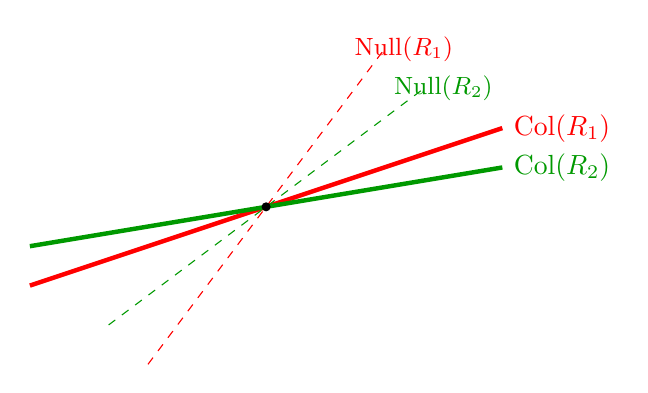
\begin{tikzpicture}[scale=0.5]
% Floor for R_1 (Col(R_1))
\draw[ultra thick, red] (-6,-2) -- (6,2) node[right]{$\operatorname{Col}(R_1)$};
% Floor for R_2 (Col(R_2))
\draw[ultra thick, green!60!black] (-6,-1) -- (6,1) node[right]{$\operatorname{Col}(R_2)$};
% Sunlight for R_1 (Null(R_1))
\draw[red, dashed] (-3,-4) -- (3,4);
\node[red] at (3.5,4) {\small $\operatorname{Null}(R_1)$};
% Sunlight for R_2 (Null(R_2))
\draw[green!60!black, dashed] (-4,-3) -- (4,3);
\node[green!60!black] at (4.5,3) {\small $\operatorname{Null}(R_2)$};
% Origin
\draw[fill=black] (0,0) circle[radius=0.1];
\end{tikzpicture}
\end{center}

\vspace{0.3em}

Key: $R_1 R_2 = 0$ means $\operatorname{Col}(R_2) \subseteq \operatorname{Null}(R_1)$.

The \x{floor} of $R_2$ lies in the \x{sunlight direction} of $R_1$ (and vice versa).

\end{frame}


\begin{frame}{Property 1: Subsums Are Projections}

\begin{prop}
Let $\{P_1, \ldots, P_k\}$ be a compatible family. For any subset $I \subseteq \{1, \ldots, k\}$, the sum $Q = \sum_{i \in I} P_i$ is a projection.
\end{prop}

\vspace{0.3em}

Proof:
$$Q^2 = \left(\sum_{i \in I} P_i\right)\left(\sum_{j \in I} P_j\right) = \sum_{i,j \in I} P_i P_j$$

Since $P_i P_j = 0$ for $i \neq j$ and $P_i^2 = P_i$:

$$Q^2 = \sum_{i \in I} P_i^2 = \sum_{i \in I} P_i = Q \quad \checkmark$$

\end{frame}

\begin{frame}{Verify with Coordinate Projections}

$P_1 + P_2 = \begin{pmatrix} 1 & 0 & 0 \\ 0 & 1 & 0 \\ 0 & 0 & 0 \end{pmatrix}$ is a projection $\checkmark$ \quad (projects onto $xy$-plane)

\vspace{0.5em}

$P_2 + P_3 = \begin{pmatrix} 0 & 0 & 0 \\ 0 & 1 & 0 \\ 0 & 0 & 1 \end{pmatrix}$ is a projection $\checkmark$ \quad (projects onto $yz$-plane)

\vspace{0.5em}

$P_1 + P_3 = \begin{pmatrix} 1 & 0 & 0 \\ 0 & 0 & 0 \\ 0 & 0 & 1 \end{pmatrix}$ is a projection $\checkmark$ \quad (projects onto $xz$-plane)

\vspace{0.5em}

$P_1 + P_2 + P_3 = I_3$ is a projection $\checkmark$

\end{frame}


\begin{frame}{Property 2: Independent Decompositions}

\begin{prop}
Let $\{P_1, \ldots, P_k\}$ be a compatible family. For any vector $\mathbf{v}$, the nonzero vectors among $\{P_1\mathbf{v}, \ldots, P_k\mathbf{v}\}$ are linearly independent.
\end{prop}

\vspace{0.3em}

Proof: Suppose $c_1 P_1\mathbf{v} + \cdots + c_k P_k\mathbf{v} = \mathbf{0}$.

\vspace{0.3em}

Left-multiply by $P_j$:

$$c_1 \underbrace{P_j P_1}_{=0}\mathbf{v} + \cdots + c_j \underbrace{P_j^2}_{=P_j}\mathbf{v} + \cdots + c_k \underbrace{P_j P_k}_{=0}\mathbf{v} = \mathbf{0}$$

$$c_j P_j\mathbf{v} = \mathbf{0}$$

If $P_j\mathbf{v} \neq \mathbf{0}$, then $c_j = 0$. \qed

\end{frame}


\begin{frame}{Direct Sum Decomposition}

If $\{P_1, \ldots, P_k\}$ is a compatible family with $P_1 + \cdots + P_k = P$, then:

$$\operatorname{Col}(P) = \operatorname{Col}(P_1) \oplus \operatorname{Col}(P_2) \oplus \cdots \oplus \operatorname{Col}(P_k)$$

\vspace{0.3em}

Every vector $P\mathbf{v}$ has a \x{unique} decomposition:

$$P\mathbf{v} = \underbrace{P_1\mathbf{v}}_{\in \operatorname{Col}(P_1)} + \underbrace{P_2\mathbf{v}}_{\in \operatorname{Col}(P_2)} + \cdots + \underbrace{P_k\mathbf{v}}_{\in \operatorname{Col}(P_k)}$$

\vspace{0.3em}

Key: $P_i P_j = 0$ ensures these subspaces are ``independent'' --- the floor of $P_i$ lies entirely in the sunlight direction of $P_j$.

\end{frame}


% ═══════════════════════════════════════
% §3 THE PROJECTION DECOMPOSITION THEOREM
% ═══════════════════════════════════════
\section{The Projection Decomposition Theorem}

\begin{frame}{The Big Question}

Compatible families seem like a very \x{special} structure. We required:

\begin{enumerate}
\item Each $P_i^2 = P_i$ \quad (projection)
\item $P_i P_j = 0$ for $i \neq j$ \quad (mutual annihilation)
\end{enumerate}

\vspace{0.5em}

Suppose we write a projection as a sum:

$$P = R_1 + R_2 + \cdots + R_k$$

We don't assume the $R_i$ are projections. We don't assume $R_i R_j = 0$.

\vspace{0.5em}

\x{Question}: Under what conditions can we \x{guarantee} that $\{R_1, \ldots, R_k\}$ is a compatible family?

\end{frame}


\begin{frame}{The Stunning Answer}

\begin{thm}[Projection Decomposition --- The Climax]
Let $P$ be a projection ($P^2 = P$). Suppose:
$$P = R_1 + R_2 + \cdots + R_k$$
where each $R_i$ is a matrix satisfying:
$$\sum_{i=1}^k \operatorname{rank}(R_i) \leq \operatorname{rank}(P)$$

Then \x{automatically}:
\begin{enumerate}
\item Each $R_i$ is a projection ($R_i^2 = R_i$)
\item $R_i R_j = 0$ for all $i \neq j$ (compatible family)
\item $\sum_{i=1}^k \operatorname{rank}(R_i) = \operatorname{rank}(P)$ (equality holds)
\end{enumerate}
\end{thm}

\end{frame}


\begin{frame}{Why Is This Remarkable?}

We \x{never assumed} the $R_i$ are projections.

\vspace{0.3em}

We \x{never assumed} $R_i R_j = 0$.

\vspace{0.5em}

The projection property and mutual annihilation \x{emerge automatically} from the rank condition alone!

\vspace{0.5em}

To check compatibility, we only need:
$$\sum \operatorname{rank}(R_i) \leq \operatorname{rank}(P)$$

\vspace{0.5em}

Key: The rank condition forces a rigid algebraic structure.

\end{frame}


\begin{frame}{Proof: Step 1 --- Introduce $R_0$}

Let $R_0 = I_n - P$. Since $P$ is a projection, $R_0$ is also a projection:

$$(I_n - P)^2 = I_n - 2P + P^2 = I_n - P = R_0 \quad \checkmark$$

\vspace{0.5em}

Now:
$$I_n = R_0 + R_1 + \cdots + R_k$$

We have reduced to the case where the pieces sum to $I_n$.

\end{frame}


\begin{frame}{Proof: Step 2 --- Count Total Rank}

By rank $=$ trace for projections (Lecture 8):

$$\operatorname{rank}(R_0) = \operatorname{trace}(R_0) = n - \operatorname{trace}(P) = n - \operatorname{rank}(P)$$

\vspace{0.5em}

Total rank of all pieces:

$$\sum_{i=0}^k \operatorname{rank}(R_i) = \underbrace{(n - \operatorname{rank}(P))}_{\operatorname{rank}(R_0)} + \underbrace{\sum_{i=1}^k \operatorname{rank}(R_i)}_{\leq \operatorname{rank}(P)} \leq n$$

\end{frame}


\begin{frame}{Proof: Step 3 --- Assemble into Block Matrices}

For each $i = 0, 1, \ldots, k$, let $r_i = \operatorname{rank}(R_i)$ and decompose:
$$R_i = U_i V_i \quad (U_i \text{ is } n \times r_i, \quad V_i \text{ is } r_i \times n)$$

\vspace{0.5em}

Collect all pieces:

$$U = \begin{pmatrix}
| & | & & | \\
U_0 & U_1 & \cdots & U_k \\
| & | & & |
\end{pmatrix}, \quad
V = \begin{pmatrix}
- & V_0 & - \\
- & V_1 & - \\
& \vdots & \\
- & V_k & -
\end{pmatrix}$$

\vspace{0.3em}

Then:
$$UV = \sum_{i=0}^k U_i V_i = \sum_{i=0}^k R_i = I_n$$

\end{frame}


\begin{frame}{Proof: Step 4 --- Forces-Square Lemma}

$U$ is $n \times s$ and $V$ is $s \times n$ where $s = \sum_{i=0}^k r_i \leq n$.

\vspace{0.5em}

We have $UV = I_n$, so $V$ is a left inverse of $U$.

\vspace{0.5em}

From Lecture 8 (full rank square matrices): since $UV = I_n$ and $s \leq n$:
$$s = n \quad \text{and} \quad VU = I_n$$

\vspace{0.5em}

(If $s < n$, then $\operatorname{rank}(UV) \leq s < n$, contradicting $UV = I_n$.)

\end{frame}


\begin{frame}{Proof: Step 5 --- Block Structure of $VU = I_n$}

$$VU = \begin{pmatrix}
V_0 U_0 & V_0 U_1 & \cdots & V_0 U_k \\
V_1 U_0 & V_1 U_1 & \cdots & V_1 U_k \\
\vdots & \vdots & \ddots & \vdots \\
V_k U_0 & V_k U_1 & \cdots & V_k U_k
\end{pmatrix} = I_n$$

\vspace{0.3em}

The $I_n$ on the right is block-diagonal: $I_{r_0} \oplus I_{r_1} \oplus \cdots \oplus I_{r_k}$.

\vspace{0.5em}

Reading off the blocks:
$$V_i U_i = I_{r_i} \quad \text{(diagonal blocks)}$$
$$V_i U_j = 0 \quad \text{for } i \neq j \quad \text{(off-diagonal blocks)}$$

\end{frame}


\begin{frame}{Proof: Step 6 --- Each $R_i$ Is a Projection}

Using $V_i U_i = I_{r_i}$:

$$R_i^2 = (U_i V_i)(U_i V_i) = U_i \underbrace{(V_i U_i)}_{= I_{r_i}} V_i = U_i V_i = R_i \quad \checkmark$$

\vspace{0.5em}

Each $R_i$ is \x{automatically} a projection!

\end{frame}


\begin{frame}{Proof: Step 7 --- Mutual Annihilation}

Using $V_i U_j = 0$ for $i \neq j$:

$$R_i R_j = (U_i V_i)(U_j V_j) = U_i \underbrace{(V_i U_j)}_{= 0} V_j = 0 \quad \checkmark$$

\vspace{0.5em}

The $R_i$ are \x{automatically} mutually annihilating!

\vspace{0.5em}

And since $s = n$: $\sum_{i=0}^k \operatorname{rank}(R_i) = n$, which gives:

$$\sum_{i=1}^k \operatorname{rank}(R_i) = n - \operatorname{rank}(R_0) = \operatorname{rank}(P) \quad \checkmark \qquad \qed$$

\end{frame}


\begin{frame}{Summary of the Proof}

The entire proof flows from one chain:

$$P = \sum R_i \;\xrightarrow{\text{add } R_0}\; I_n = \sum R_i \;\xrightarrow{\text{factor}}\; UV = I_n$$
$$\xrightarrow{s \leq n}\; VU = I_n \;\xrightarrow{\text{blocks}}\; V_i U_j = \delta_{ij} I_{r_i}$$

\vspace{0.5em}

From $V_i U_j = \delta_{ij} I_{r_i}$, we read off:
\begin{itemize}
\item $R_i^2 = R_i$ (from diagonal blocks)
\item $R_i R_j = 0$ (from off-diagonal blocks)
\end{itemize}

\vspace{0.5em}

Key: The rank condition $\sum \operatorname{rank}(R_i) \leq \operatorname{rank}(P)$ forces $s \leq n$, which forces $VU = I_n$, which forces everything.

\end{frame}


\begin{frame}{Exercise: Verify the Rank Condition}

$$P = \underbrace{\begin{pmatrix} 0 & 0 & 0 \\ -1 & 1 & 0 \\ 0 & 0 & 0 \end{pmatrix}}_{\operatorname{rank} = 1} + \underbrace{\begin{pmatrix} 0 & 0 & 0 \\ 0 & 0 & 0 \\ -1 & 0 & 1 \end{pmatrix}}_{\operatorname{rank} = 1}$$

\vspace{0.3em}

$\sum \operatorname{rank}(R_i) = 1 + 1 = 2 = \operatorname{rank}(P)$ $\checkmark$

\vspace{0.5em}

By the theorem: $R_1, R_2$ are automatically projections and $R_1 R_2 = 0$.

We get this \x{for free} --- no need to multiply matrices!

\end{frame}


\begin{frame}{Exercise: When the Rank Condition Fails}

Consider the same $P$ but a \x{different} decomposition:

$$P = \underbrace{\begin{pmatrix} 0 & 0 & 0 \\ -1/2 & 1/2 & 0 \\ -1 & 0 & 1 \end{pmatrix}}_{\operatorname{rank} = 2} + \underbrace{\begin{pmatrix} 0 & 0 & 0 \\ -1/2 & 1/2 & 0 \\ 0 & 0 & 0 \end{pmatrix}}_{\operatorname{rank} = 1}$$

\vspace{0.3em}

$\sum \operatorname{rank}(R_i) = 2 + 1 = 3 > 2 = \operatorname{rank}(P)$

\vspace{0.5em}

The rank condition \x{fails}. And indeed, the first piece is \x{not} a projection.

The theorem does not apply --- and the conclusion fails!

\end{frame}


% ═══════════════════════════════════════
% §4 APPLICATIONS
% ═══════════════════════════════════════
\section{Applications}

\begin{frame}{Application 1: Cross-Filling Produces Compatible Projections}

\begin{cor}
Let $P$ be a projection. Cross-fill $P = R_1 + \cdots + R_r$ into rank-1 pieces. Then $\{R_1, \ldots, R_r\}$ is a compatible family of rank-1 projections.
\end{cor}

\vspace{0.5em}

Proof: By construction, each $R_i$ has rank 1, and:

$$\sum_{i=1}^r \operatorname{rank}(R_i) = r = \operatorname{rank}(P)$$

Apply the Projection Decomposition Theorem. \qed

\vspace{0.5em}

In Lecture 8, we proved this directly. The theorem provides a \x{second, more powerful proof} that generalizes far beyond cross-filling.

\end{frame}


\begin{frame}{Application 2: Rank-1 Projections Have $r_i^T c_j = \delta_{ij}$}

Cross-filling a projection $P$ of rank $r$:

$$P = \underbrace{c_1 r_1^T}_{R_1} + \underbrace{c_2 r_2^T}_{R_2} + \cdots + \underbrace{c_r r_r^T}_{R_r}$$

\vspace{0.3em}

Write as $P = UV$ where:
$$U = \begin{pmatrix}
| & & | \\
c_1 & \cdots & c_r \\
| & & |
\end{pmatrix}, \quad
V = \begin{pmatrix}
- & r_1^T & - \\
& \vdots & \\
- & r_r^T & -
\end{pmatrix}$$

\vspace{0.3em}

The theorem gives $VU = I_r$, which means:

$$r_i^T c_j = \begin{cases} 1 & i = j \\ 0 & i \neq j \end{cases}$$

\end{frame}

\begin{frame}{Verify with Our Example}

$$R_1 = \begin{pmatrix} 0 \\ 1 \\ 0 \end{pmatrix}\begin{pmatrix} -1 & 1 & 0 \end{pmatrix}, \quad R_2 = \begin{pmatrix} 0 \\ 0 \\ 1 \end{pmatrix}\begin{pmatrix} -1 & 0 & 1 \end{pmatrix}$$

\vspace{0.3em}

Check $r_i^T c_j = \delta_{ij}$:

\vspace{0.3em}

$r_1^T c_1 = \begin{pmatrix} -1 & 1 & 0 \end{pmatrix}\begin{pmatrix} 0 \\ 1 \\ 0 \end{pmatrix} = 1$ $\checkmark$ \qquad
$r_1^T c_2 = \begin{pmatrix} -1 & 1 & 0 \end{pmatrix}\begin{pmatrix} 0 \\ 0 \\ 1 \end{pmatrix} = 0$ $\checkmark$

\vspace{0.3em}

$r_2^T c_1 = \begin{pmatrix} -1 & 0 & 1 \end{pmatrix}\begin{pmatrix} 0 \\ 1 \\ 0 \end{pmatrix} = 0$ $\checkmark$ \qquad
$r_2^T c_2 = \begin{pmatrix} -1 & 0 & 1 \end{pmatrix}\begin{pmatrix} 0 \\ 0 \\ 1 \end{pmatrix} = 1$ $\checkmark$

\end{frame}


\begin{frame}{Application 3: Inner Cross-Filling --- Motivation}

Cross-filling decomposes $P$ directly into rank-1 pieces.

\vspace{0.5em}

But what if $P$ has a \x{factored form}?

$$P = M_1 M_2 \cdots M_k$$

\vspace{0.5em}

Idea: Instead of cross-filling the $n \times n$ matrix $P$, cross-fill a \x{smaller factor} inside $P$.

\vspace{0.5em}

The Projection Decomposition Theorem will guarantee that the resulting pieces still form a compatible family!

\end{frame}


\begin{frame}{Inner Cross-Filling: Theorem}

\begin{thm}[Inner Cross-Filling]
Let $P$ be a projection. Suppose $P = M_1 M_2 \cdots M_k$ where $\operatorname{rank}(P) = \operatorname{rank}(M_i)$ for some factor $M_i$.

Cross-fill $M_i = Q_1 + Q_2 + \cdots + Q_s$ into rank-1 pieces. Define:
$$S_j = M_1 \cdots M_{i-1} \, Q_j \, M_{i+1} \cdots M_k$$

Then $P = S_1 + \cdots + S_s$ is a compatible family of projections.
\end{thm}

\end{frame}


\begin{frame}{Inner Cross-Filling: Why It Works}

Clearly $P = \sum_j S_j$ (distribute the product over the sum).

\vspace{0.5em}

For rank:
$$\operatorname{rank}(S_j) \leq \operatorname{rank}(Q_j) = 1$$

$$\sum_j \operatorname{rank}(S_j) \leq \sum_j \operatorname{rank}(Q_j) = \operatorname{rank}(M_i) = \operatorname{rank}(P)$$

\vspace{0.5em}

By the Projection Decomposition Theorem: each $S_j$ is a projection and $S_j S_l = 0$ for $j \neq l$. \qed

\vspace{0.5em}

Key: We decompose an \x{inner factor} $M_i$ rather than $P$ itself. The outer factors are ``carried along for the ride.''

\end{frame}


\begin{frame}{Inner Cross-Filling: Example}

Let $P = \begin{pmatrix} 1 & 0 & 0 \\ 0 & 1 & 0 \\ 0 & 0 & 0 \end{pmatrix}$ (projection onto $xy$-plane).

\vspace{0.3em}

Write $P = U \cdot I_2 \cdot V$ where:

$$U = \begin{pmatrix} 1 & 0 \\ 0 & 1 \\ 0 & 0 \end{pmatrix}, \quad V = \begin{pmatrix} 1 & 0 & 0 \\ 0 & 1 & 0 \end{pmatrix}$$

\vspace{0.3em}

$\operatorname{rank}(P) = 2 = \operatorname{rank}(I_2)$ $\checkmark$. Cross-fill $I_2$:

$$I_2 = \underbrace{\begin{pmatrix} 1 & 0 \\ 0 & 0 \end{pmatrix}}_{Q_1} + \underbrace{\begin{pmatrix} 0 & 0 \\ 0 & 1 \end{pmatrix}}_{Q_2}$$

\end{frame}


\begin{frame}{Inner Cross-Filling: Example (continued)}

$$S_1 = UQ_1V = \begin{pmatrix} 1 & 0 \\ 0 & 1 \\ 0 & 0 \end{pmatrix}\begin{pmatrix} 1 & 0 \\ 0 & 0 \end{pmatrix}\begin{pmatrix} 1 & 0 & 0 \\ 0 & 1 & 0 \end{pmatrix} = \begin{pmatrix} 1 & 0 & 0 \\ 0 & 0 & 0 \\ 0 & 0 & 0 \end{pmatrix}$$

\vspace{0.3em}

$$S_2 = UQ_2V = \begin{pmatrix} 1 & 0 \\ 0 & 1 \\ 0 & 0 \end{pmatrix}\begin{pmatrix} 0 & 0 \\ 0 & 1 \end{pmatrix}\begin{pmatrix} 1 & 0 & 0 \\ 0 & 1 & 0 \end{pmatrix} = \begin{pmatrix} 0 & 0 & 0 \\ 0 & 1 & 0 \\ 0 & 0 & 0 \end{pmatrix}$$

\vspace{0.5em}

$S_1^2 = S_1$ $\checkmark$, \; $S_2^2 = S_2$ $\checkmark$, \; $S_1 S_2 = 0$ $\checkmark$

\vspace{0.3em}

We decomposed the $3 \times 3$ projection by cross-filling the \x{smaller} $2 \times 2$ identity!

\end{frame}


% ═══════════════════════════════════════
% §5 INNER DIAGONAL CROSS-FILLING
% ═══════════════════════════════════════
\section{Inner Diagonal Cross-Filling}

\begin{frame}{Combining Inner and Diagonal Cross-Filling}

From Lecture 8: diagonal cross-filling decomposes an orthogonal projection $P$ into rank-1 \x{orthogonal} projections.

\vspace{0.5em}

From \S4: inner cross-filling lets us decompose a \x{smaller factor} inside $P$.

\vspace{0.5em}

\x{Question}: Can we combine these ideas?

\vspace{0.5em}

If $P = UMU^T$ where $M$ is a \x{small symmetric} matrix, can we diagonally cross-fill $M$ and get orthogonal projections?

\end{frame}


\begin{frame}{The Setup: $P = UMU^T$}

Suppose an orthogonal projection has the form:
$$P = UMU^T$$

where:
\begin{itemize}
\item $U$ is $n \times r$ with \x{full column rank} ($\operatorname{rank}(U) = r$)
\item $M$ is $r \times r$ and \x{symmetric} ($M = M^T$)
\item $\operatorname{rank}(P) = \operatorname{rank}(M)$
\end{itemize}

\vspace{0.5em}

Key observation: $M$ is a \x{much smaller} matrix than $P$.

\vspace{0.3em}

$M$ is $r \times r$ vs.\ $P$ is $n \times n$. When $r \ll n$, this is a big difference!

\end{frame}


\begin{frame}{Inner Diagonal Cross-Filling: Theorem}

\begin{thm}[Inner Diagonal Cross-Filling]
Let $P = UMU^T$ be an orthogonal projection where $M$ is $r \times r$ symmetric and $\operatorname{rank}(P) = \operatorname{rank}(M)$.

Diagonally cross-fill $M$:
$$M = Q_1 + Q_2 + \cdots + Q_r$$

Define $R_j = UQ_jU^T$. Then:
\begin{enumerate}
\item $P = R_1 + R_2 + \cdots + R_r$
\item Each $R_j$ is a rank-1 \x{orthogonal} projection
\item $\{R_1, \ldots, R_r\}$ is a compatible family
\end{enumerate}
\end{thm}

\end{frame}


\begin{frame}{Why It Works}

\x{Step 1}: $\sum R_j = \sum UQ_jU^T = U\left(\sum Q_j\right)U^T = UMU^T = P$ $\checkmark$

\vspace{0.5em}

\x{Step 2} (rank): $\operatorname{rank}(R_j) \leq \operatorname{rank}(Q_j) = 1$, so:
$$\sum_j \operatorname{rank}(R_j) \leq \sum_j \operatorname{rank}(Q_j) = \operatorname{rank}(M) = \operatorname{rank}(P)$$

By PDT: each $R_j$ is a projection and $R_j R_l = 0$. $\checkmark$

\vspace{0.5em}

\x{Step 3} (symmetry): Since $Q_j$ is symmetric (diagonal pivot preserves symmetry):
$$R_j^T = (UQ_jU^T)^T = UQ_j^TU^T = UQ_jU^T = R_j \;\checkmark$$

Each $R_j$ is a projection \x{and} symmetric $\implies$ orthogonal projection. \qed

\end{frame}


\begin{frame}{The Key Example: Orthogonal Projection Formula}

The most important case: the orthogonal projection onto $\operatorname{Col}(B)$:

$$P = B(B^TB)^{-1}B^T$$

\vspace{0.5em}

This has the form $P = UMU^T$ with:

\vspace{0.3em}

\begin{itemize}
\item $U = B$ \quad ($n \times r$, full column rank)
\item $M = (B^TB)^{-1}$ \quad ($r \times r$, symmetric $\checkmark$)
\item $\operatorname{rank}(M) = r = \operatorname{rank}(P)$ $\checkmark$
\end{itemize}

\vspace{0.5em}

Instead of diagonally cross-filling the $n \times n$ matrix $P$, we cross-fill the \x{small} $r \times r$ matrix $(B^TB)^{-1}$!

\end{frame}


\begin{frame}{Efficiency Comparison}

\begin{center}
\begin{tabular}{lcc}
\textbf{Method} & \textbf{Matrix size} & \textbf{Cost per step} \\
\hline
Direct diagonal cross-filling of $P$ & $n \times n$ & $O(n^2)$ \\
Inner diagonal cross-filling of $(B^TB)^{-1}$ & $r \times r$ & $O(r^2)$ \\
\end{tabular}
\end{center}

\vspace{0.5em}

When $r \ll n$: inner diagonal cross-filling is \x{much faster}.

\vspace{0.5em}

Example: $B$ is $100 \times 3$ (3 basis vectors in $\mathbb{R}^{100}$).

\vspace{0.3em}

Direct: cross-fill a $100 \times 100$ matrix.

Inner: cross-fill a $3 \times 3$ matrix!

\end{frame}


\begin{frame}{Example: Setup}

Let $B = \begin{pmatrix} 1 & 0 \\ 1 & 1 \\ 1 & 2 \end{pmatrix}$ \quad ($3 \times 2$, full column rank).

\vspace{0.5em}

\x{Step 1}: Compute $B^TB$ and $(B^TB)^{-1}$:

$$B^TB = \begin{pmatrix} 1 & 1 & 1 \\ 0 & 1 & 2 \end{pmatrix}\begin{pmatrix} 1 & 0 \\ 1 & 1 \\ 1 & 2 \end{pmatrix} = \begin{pmatrix} 3 & 3 \\ 3 & 5 \end{pmatrix}$$

\vspace{0.3em}

$\det(B^TB) = 15 - 9 = 6$

$$(B^TB)^{-1} = \frac{1}{6}\begin{pmatrix} 5 & -3 \\ -3 & 3 \end{pmatrix}$$

This is our $2 \times 2$ symmetric matrix $M$ to cross-fill!

\end{frame}


\begin{frame}{Example: Diagonal Cross-Fill $M$}

$$M = (B^TB)^{-1} = \frac{1}{6}\begin{pmatrix} 5 & -3 \\ -3 & 3 \end{pmatrix}$$

\x{Pivot $(1,1)$}, value $= \frac{5}{6}$:

$$Q_1 = \frac{1}{5/6} \cdot \frac{1}{6}\begin{pmatrix} 5 \\ -3 \end{pmatrix} \cdot \frac{1}{6}\begin{pmatrix} 5 & -3 \end{pmatrix} = \frac{1}{30}\begin{pmatrix} 25 & -15 \\ -15 & 9 \end{pmatrix}$$

\vspace{0.3em}

Remainder:
$$Q_2 = M - Q_1 = \frac{1}{6}\begin{pmatrix} 5 & -3 \\ -3 & 3 \end{pmatrix} - \frac{1}{30}\begin{pmatrix} 25 & -15 \\ -15 & 9 \end{pmatrix} = \frac{1}{5}\begin{pmatrix} 0 & 0 \\ 0 & 1 \end{pmatrix}$$

Both $Q_1 = Q_1^T$ $\checkmark$ and $Q_2 = Q_2^T$ $\checkmark$ (diagonal pivots preserve symmetry!)

\end{frame}


\begin{frame}{Example: Compute $R_1 = BQ_1B^T$}

$$BQ_1 = \begin{pmatrix} 1 & 0 \\ 1 & 1 \\ 1 & 2 \end{pmatrix}\frac{1}{30}\begin{pmatrix} 25 & -15 \\ -15 & 9 \end{pmatrix} = \frac{1}{30}\begin{pmatrix} 25 & -15 \\ 10 & -6 \\ -5 & 3 \end{pmatrix}$$

\vspace{0.3em}

$$R_1 = BQ_1B^T = \frac{1}{30}\begin{pmatrix} 25 & -15 \\ 10 & -6 \\ -5 & 3 \end{pmatrix}\begin{pmatrix} 1 & 1 & 1 \\ 0 & 1 & 2 \end{pmatrix} = \frac{1}{30}\begin{pmatrix} 25 & 10 & -5 \\ 10 & 4 & -2 \\ -5 & -2 & 1 \end{pmatrix}$$

\vspace{0.3em}

$R_1 = R_1^T$ $\checkmark$, \; $\operatorname{rank}(R_1) = 1$ $\checkmark$, \; $\operatorname{trace}(R_1) = 1$ $\checkmark$

\end{frame}


\begin{frame}{Example: Compute $R_2 = BQ_2B^T$}

$$BQ_2 = \begin{pmatrix} 1 & 0 \\ 1 & 1 \\ 1 & 2 \end{pmatrix}\frac{1}{5}\begin{pmatrix} 0 & 0 \\ 0 & 1 \end{pmatrix} = \frac{1}{5}\begin{pmatrix} 0 & 0 \\ 0 & 1 \\ 0 & 2 \end{pmatrix}$$

\vspace{0.3em}

$$R_2 = BQ_2B^T = \frac{1}{5}\begin{pmatrix} 0 & 0 \\ 0 & 1 \\ 0 & 2 \end{pmatrix}\begin{pmatrix} 1 & 1 & 1 \\ 0 & 1 & 2 \end{pmatrix} = \frac{1}{5}\begin{pmatrix} 0 & 0 & 0 \\ 0 & 1 & 2 \\ 0 & 2 & 4 \end{pmatrix}$$

\vspace{0.3em}

$R_2 = R_2^T$ $\checkmark$, \; $\operatorname{rank}(R_2) = 1$ $\checkmark$, \; $\operatorname{trace}(R_2) = 1$ $\checkmark$

\end{frame}


\begin{frame}{Example: Verification}

\x{Compatibility}: $R_1 R_2 = 0$ $\checkmark$ (direct computation)

\vspace{0.5em}

\x{Sum}:
$$R_1 + R_2 = \frac{1}{30}\begin{pmatrix} 25 & 10 & -5 \\ 10 & 4 & -2 \\ -5 & -2 & 1 \end{pmatrix} + \frac{1}{5}\begin{pmatrix} 0 & 0 & 0 \\ 0 & 1 & 2 \\ 0 & 2 & 4 \end{pmatrix}$$

$$= \frac{1}{6}\begin{pmatrix} 5 & 2 & -1 \\ 2 & 2 & 2 \\ -1 & 2 & 5 \end{pmatrix} = P \;\checkmark$$

\vspace{0.3em}

We decomposed a $3 \times 3$ orthogonal projection by cross-filling a $2 \times 2$ matrix!

\end{frame}


\begin{frame}{The Real Payoff: Orthogonal Basis}

Each $Q_j$ from diagonal cross-filling has the form $Q_j = \frac{1}{q_{jj}} \mathbf{d}_j \mathbf{d}_j^T$.

\vspace{0.3em}

So: $R_j = BQ_jB^T = \frac{1}{q_{jj}} (B\mathbf{d}_j)(B\mathbf{d}_j)^T$

\vspace{0.5em}

Since $R_i R_j = 0$ for $i \neq j$:
$$\frac{1}{q_{ii} q_{jj}} (B\mathbf{d}_i) \underbrace{(\mathbf{d}_i^T B^T B \mathbf{d}_j)}_{=\;?} (B\mathbf{d}_j)^T = 0$$

This forces $(B\mathbf{d}_i)^T(B\mathbf{d}_j) = \mathbf{d}_i^T B^T B \mathbf{d}_j = 0$.

\vspace{0.5em}

The vectors $B\mathbf{d}_1, \ldots, B\mathbf{d}_r$ are \x{mutually orthogonal} and span $\operatorname{Col}(B)$!

\end{frame}


\begin{frame}{Extracting the Orthogonal Basis}

Read $\mathbf{d}_j$ from each $Q_j$ and multiply by $B$:

\vspace{0.3em}

$$\mathbf{d}_1 \propto \begin{pmatrix} 5 \\ -3 \end{pmatrix} \implies B\mathbf{d}_1 = \begin{pmatrix} 5 \\ 2 \\ -1 \end{pmatrix} \qquad \mathbf{d}_2 \propto \begin{pmatrix} 0 \\ 1 \end{pmatrix} \implies B\mathbf{d}_2 = \begin{pmatrix} 0 \\ 1 \\ 2 \end{pmatrix}$$

\vspace{0.3em}

\x{Check orthogonality}: $(5)(0) + (2)(1) + (-1)(2) = 0$ $\checkmark$

\vspace{0.3em}

$\left\{\begin{pmatrix} 5 \\ 2 \\ -1 \end{pmatrix}, \begin{pmatrix} 0 \\ 1 \\ 2 \end{pmatrix}\right\}$ is an \x{orthogonal basis} for $\operatorname{Col}(B)$!

\end{frame}


\begin{frame}{What $\mathbf{d}_j$ Tells You}

$\mathbf{d}_j$ gives the \x{coefficients} for combining original columns of $B$ into orthogonal vectors:

\vspace{0.5em}

$$\mathbf{d}_1 = \begin{pmatrix} 5 \\ -3 \end{pmatrix}: \quad 5 \cdot \begin{pmatrix} 1 \\ 1 \\ 1 \end{pmatrix} + (-3) \cdot \begin{pmatrix} 0 \\ 1 \\ 2 \end{pmatrix} = \begin{pmatrix} 5 \\ 2 \\ -1 \end{pmatrix}$$

$$\mathbf{d}_2 = \begin{pmatrix} 0 \\ 1 \end{pmatrix}: \quad 0 \cdot \begin{pmatrix} 1 \\ 1 \\ 1 \end{pmatrix} + 1 \cdot \begin{pmatrix} 0 \\ 1 \\ 2 \end{pmatrix} = \begin{pmatrix} 0 \\ 1 \\ 2 \end{pmatrix}$$

\vspace{0.5em}

The cross-filling of $(B^TB)^{-1}$ computes these coefficients \x{automatically}.

No Gram--Schmidt needed!

\end{frame}


\begin{frame}{Summary: Inner Diagonal Cross-Filling Algorithm}

Given a basis $\{\mathbf{b}_1, \ldots, \mathbf{b}_r\}$ for a subspace $W$ (columns of $B$):

\vspace{0.5em}

\begin{enumerate}
\item Compute $(B^TB)^{-1}$ \quad (an $r \times r$ symmetric matrix)
\item Diagonally cross-fill $(B^TB)^{-1}$: at each step, read column $\mathbf{d}_j$ at the pivot
\item Compute $B\mathbf{d}_j$ $\to$ orthogonal basis vector for $W$
\item (Optional) Normalize: $\mathbf{v}_j = B\mathbf{d}_j / \|B\mathbf{d}_j\|$ for orthonormal basis
\end{enumerate}

\vspace{0.5em}

\x{Why it works}: The Projection Decomposition Theorem guarantees mutual orthogonality of the $B\mathbf{d}_j$ automatically.

\end{frame}


% ═══════════════════════════════════════
% §6 SPECTRAL DECOMPOSITION PREVIEW
% ═══════════════════════════════════════
\section{Preview: Spectral Decomposition}

\begin{frame}{Compatible Families and Matrix Powers}

Suppose $\{P_1, P_2, \ldots, P_n\}$ is a compatible family with $P_1 + \cdots + P_n = I$.

\vspace{0.3em}

If $A = \lambda_1 P_1 + \lambda_2 P_2 + \cdots + \lambda_n P_n$, then:

$$AB = (\lambda_1 P_1 + \cdots)(\mu_1 P_1 + \cdots) = \lambda_1\mu_1 P_1 + \cdots + \lambda_n\mu_n P_n$$

because $P_i P_j = 0$ for $i \neq j$.

\vspace{0.5em}

In particular:

$$A^k = \lambda_1^k P_1 + \lambda_2^k P_2 + \cdots + \lambda_n^k P_n$$

\end{frame}


\begin{frame}{Example: Computing Matrix Powers}

$$\begin{pmatrix} 2 & 1 \\ 1 & 2 \end{pmatrix} = 1 \cdot \underbrace{\frac{1}{2}\begin{pmatrix} 1 & -1 \\ -1 & 1 \end{pmatrix}}_{P_1} + 3 \cdot \underbrace{\frac{1}{2}\begin{pmatrix} 1 & 1 \\ 1 & 1 \end{pmatrix}}_{P_2}$$

\vspace{0.3em}

$P_1^2 = P_1$ $\checkmark$, \; $P_2^2 = P_2$ $\checkmark$, \; $P_1 P_2 = 0$ $\checkmark$, \; $P_1 + P_2 = I_2$ $\checkmark$

\vspace{0.5em}

Therefore:

$$\begin{pmatrix} 2 & 1 \\ 1 & 2 \end{pmatrix}^n = 1^n P_1 + 3^n P_2 = \frac{1}{2}\begin{pmatrix} 1 + 3^n & -1 + 3^n \\ -1 + 3^n & 1 + 3^n \end{pmatrix}$$

\vspace{0.3em}

This is the main idea behind \x{spectral decomposition} (Chapter 5).

\end{frame}


% ═══════════════════════════════════════
% §7 SUMMARY
% ═══════════════════════════════════════
\section{Summary}

\begin{frame}{Key Results}

\begin{enumerate}
\item \x{Compatible Families}: Projections $\{P_1, \ldots, P_k\}$ with $P_iP_j = 0$ --- subsums are projections, vector decompositions are linearly independent.

\vspace{0.3em}

\item \x{Projection Decomposition Theorem}: If $P = \sum R_i$ with $\sum \operatorname{rank}(R_i) \leq \operatorname{rank}(P)$, then each $R_i$ is a projection and $R_iR_j = 0$ --- \x{automatically}.

\vspace{0.3em}

\item \x{Cross-Filling}: Special case of the theorem --- always produces compatible families.

\vspace{0.3em}

\item \x{Inner Cross-Filling}: Decompose an inner factor of $P$ --- the outer factors carry along.

\vspace{0.3em}

\item \x{Inner Diagonal Cross-Filling}: For $P = UMU^T$ with $M$ symmetric, diagonally cross-fill the small $M$ $\to$ orthogonal sub-projections. Produces orthogonal basis via $B\mathbf{d}_j$.
\end{enumerate}

\end{frame}


\begin{frame}{Looking Ahead: Lecture 10}

We have powerful tools for \x{decomposing} projections. But we still haven't answered:

\vspace{0.5em}

\x{Given a desired floor $W$ and sunlight direction $S$, how do we construct $P$?}

\vspace{0.5em}

In Lecture 10:
\begin{itemize}
\item A projection is \x{uniquely determined} by $\operatorname{Col}(P)$ and $\operatorname{Null}(P)$
\item Construction formula: $P = B(AB)^{-1}A$
\item Orthogonal projection formula: $P = B(B^TB)^{-1}B^T$ (proof)
\item Least squares and applications
\end{itemize}

\end{frame}


\end{document}
